% =====================================================================================================
\section{Hardware Results}\label{sec:hwresults}
\subsection{Verification}\label{sec:verification}
A Python golden model is the referee for every RTL stage; its Ascon passes all 1089 official known-answer tests, as does the RTL core. Every RTL module has a cocotb testbench with random idle cycles and back-pressure that reports the first mismatch, and the complete encoders are byte-exact with the model for every level and for one, two and four lanes, in Icarus Verilog and in Vivado's simulator. Every defect found received a regression test and a root cause.

\subsection{Cycles, area and timing}
In RTL simulation the cycle counts of E0--E4 differ by at most \MaxExtraCycles{} cycles per frame, which is handshake noise: as Proposition~\ref{prop:supply} predicts, encryption costs no cycles. Above the floor of 1.5 cycles per pixel the only cost of a single pipeline is filling the first MCU row, $c_1(r) = 1.5 + \FillA/r$ for $r$ MCU rows (\CppVGA{} at 640$\times$480). One, two and four lanes reach \RtlOneLaneMpix, \RtlTwoLanesMpix{} and \RtlFourLanesMpix\,Mpixel/s at 100\,MHz, against the bounds \BoundOneMpix, \BoundTwoMpix{} and \BoundFourMpix{} of~\eqref{eq:lanes}; E5, with one restart per MCU, costs a few per cent.

% generated by paper/make_assets.py from paper/data -- do not edit
\begin{table}[t]
\caption{Resources on the xc7z020 (53\,200 LUT, 106\,400 FF, 140 BRAM36, 220 DSP). Source: Vivado post-route, out of context, 100\,MHz with I/O delays of 20\,\% of the period, WNS +0.630\,ns.}
\label{tab:resources}
\centering\small
\resizebox{\columnwidth}{!}{%
\begin{tabular}{lrrrr}
\toprule
Block & LUT & FF & BRAM36 & DSP \\
\midrule
Encoder (all) & 4785 (9.0\%) & 3051 (2.9\%) & 25.5 (18.2\%) & 23 (10.4\%) \\
\quad colour conversion + line buffers & 459 & 220 & 25 & 0 \\
\quad DCT and quantizer & 806 & 69 & 0 & 22 \\
\quad zig-zag, Huffman, packing & 717 & 323 & 0 & 0 \\
\quad keystream generator (Ascon) & 949 & 851 & 0 & 0 \\
\quad tag unit (Ascon) & 1358 & 1072 & 0 & 0 \\
\quad selective encryption & 82 & 24 & 0 & 0 \\
\quad AXI-Lite registers & 392 & 451 & 0 & 0 \\
\bottomrule
\end{tabular}}
\end{table}

After place and route the single pipeline meets \TopMhz\,MHz on the xc7z020 (WNS $+$\TopWns\,ns, out of context) with \TopLuts{} LUTs (\TopLutPct\,\% of the device, Table~\ref{tab:resources}); the two Ascon instances take \CryptoLutShare\,\% of them and the selective-encryption stage is tiny. With switching activity from simulating a real frame it draws about \SaifTopMw\,mW. Two lanes take \TwoLanesLuts{} LUTs and four lanes \FourLanesLuts{}; E5 adds no BRAM or DSP. Out of context one, two and four lanes also meet 150\,MHz (WNS \TopWnsAtOneFifty, \LanesTwoWnsAtOneFifty{} and \LanesFourWnsAtOneFifty\,ns). The complete PYNQ-Z2 systems close timing: one and two lanes at \OverlayMhz\,MHz, four lanes at \OverlayLanesFourMhz\,MHz with \OverlayLanesFourLuts{} LUTs (\OverlayLanesFourLutPct\,\% of the device).

% generated by paper/make_assets.py from paper/data -- do not edit
\begin{table}[t]
\caption{Comparison with published FPGA designs. Their numbers are as reported by each source; ours are
post-route (Table~\ref{tab:resources}) with throughput from the RTL cycle count. Mpx/s: million pixels per second.}
\label{tab:compare}
\centering\small
\resizebox{\columnwidth}{!}{%
\begin{tabular}{llrrrrrl}
\toprule
Design & Device & LUT & BRAM & DSP & MHz & Mpx/s & Crypto \\
\midrule
Ours: encoder & Zynq-7020 & 5{,}039 & 24.5 & 23 & 100 & 61 & sel.\ AEAD \\
Ours: one Ascon & Zynq-7020 & 860--969 & 0 & 0 & 100 & -- & AEAD core \\
logiJPGE~\cite{logijpge} & Zynq-7020 & 3{,}240 & 16 & 30 & 150 & 150 & none \\
CAST JPEG-E-S~\cite{castjpeg} & Artix-7 & 3{,}069 & 2 & 16 & 166 & -- & none \\
Khairallah~\cite{khairallah2023} & Artix-7 & 1{,}031 & 0 & 0 & 200 & -- & MAC \\
Kurian~\cite{kurian2025} & Artix-7 & 5{,}335 & 32 & 0 & 100 & -- & AEAD \\
\bottomrule
\end{tabular}}
\end{table}

\textit{Comparison.} Table~\ref{tab:compare} sets the design against published FPGA work. Each Ascon core (\AsconLutMin--\AsconLutMax{} LUTs) is as small as the round-per-cycle Ascon cores of~\cite{khairallah2023}; the commercial encoders~\cite{logijpge,castjpeg} use less block RAM and no cryptography. Per thousand LUTs, one and four lanes give \HeTopPerKlut{} and \HeFourPerKlut\,Mpixel/s against \HeKishorePerKlut{} for the scrambling encoder of Kishore et al.~\cite{kishore2015}.

\subsection{Board evaluation}\label{sec:board}
% generated by paper/make_assets.py from paper/data -- do not edit
\begin{table*}[t]
\caption{On the PYNQ-Z2 (24 Oct 2026): the final board images, each at the clock it was built for, and the same
function on the board's ARM Cortex-A9. Bit-exact: every frame of every level compared byte for byte (scan and tag)
with the golden model running on the board (58 frames in all). Fabric: START to DONE from
the encoder's CYCLES register for one 640$\times$480 frame (Mpixel/s in brackets); wait: share of those cycles in
which the encoder could take a pixel but the DMA had none, mostly because the Python driver starts the DMA after the encoder. Frame: a complete authenticated JPEG with headers (and
for E5 the segment order) on the ARM, the pixels already in the DMA buffer as a camera would leave them, median of
50 frames (frames/s in brackets). ARM rows: median of 30 frames; ``file'' encrypts the whole JPEG, so it does not
play without the key.}
\label{tab:board}
\centering\small\setlength{\tabcolsep}{4pt}
\resizebox{\textwidth}{!}{%
\begin{tabular}{lrlrrrr}
\toprule
Encoder & MHz & Bit-exact & Fabric, ms & Wait (\%) & E2 frame, ms & E5 frame, ms \\
\midrule
4 lanes & 125 & E0--E5 & 1.97 (156) & 31 & 5.9 (169) & 8.4 (119) \\
2 lanes & 100 & E0--E5 & 3.06 (100) & 21 & 7.0 (144) & 9.8 (102) \\
1 lane & 100 & E0--E4 & 5.34 (58) & 12 & 9.2 (108) & -- \\
\midrule
ARM, ours in C, 1 core & -- & E0--E5 & -- & -- & 114.2 (8.8) & 133.0 (7.5) \\
ARM, ours in C, 2 cores & -- & E0--E5 & -- & -- & 61.6 (16.2) & 74.8 (13.4) \\
ARM, libjpeg-turbo, no security & -- & -- & -- & -- & 28.8 (34.8) & -- \\
ARM, libjpeg-turbo + Ascon (file) & -- & -- & -- & -- & 31.7 (31.5) & -- \\
ARM, libjpeg-turbo + AES-GCM (file) & -- & -- & -- & -- & 31.9 (31.3) & -- \\
\bottomrule
\end{tabular}}
\end{table*}

\begin{figure}[t]
\centering
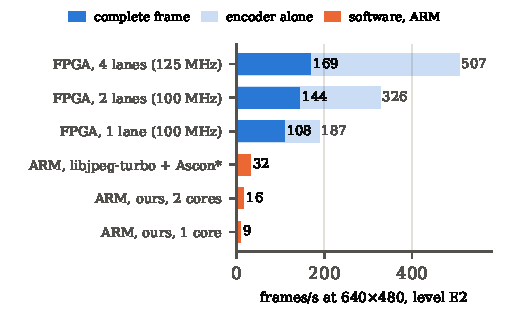
\includegraphics[width=\columnwidth]{figures/fig_board_fps.pdf}
\caption{Measured on the PYNQ-Z2: authenticated 640$\times$480 frames per second (E2) of the three board images, each at the clock it was built for, and of software on the board's two Cortex-A9 cores. Light: the encoder alone, START to DONE from its cycle counter. *Encrypts the whole file, so it does not play without the key.}
\label{fig:boardfps}
\end{figure}
The board evaluation has four parts, all scripted and rehearsed against an emulation of the bitstream: (A1) a bit-exact gate that encodes frames in every level on the fabric and compares every byte and tag with the golden model running on the board; (A2) the fabric's own time from its cycle counters and the time of a complete frame; (A3) the same function on the board's processing system; and (A4) energy per frame. Table~\ref{tab:board} gives the results.

\textit{Correctness.} All \BdImages{} board images, one, two and four lanes, are bit-exact with the golden model in every level they implement (\BdFramesTotal{} frames, every scan byte and tag). The board thus confirms Lemma~\ref{lem:format} and the lane, E5 and tag logic on silicon.

\textit{Speed.} The images count the clocks from start to done and, among them, the clocks in which the encoder could take a pixel but the DMA had none. Without those waits the counts equal the RTL simulation to within \BdBusyVsRtlMaxPct\,\% for every image: four lanes at \BdFourMhz\,MHz encode a 640$\times$480 frame in \BdFourBusyMs\,ms (\BdFourBusyMpix\,Mpixel/s), and the encoding clocks of E0--E4 differ by at most \BdFourBusySpreadClk{} per frame, so encryption costs no time on silicon either. The waits are almost the same for every image, \BdWaitMsMin--\BdWaitMsMax\,ms per frame, because our Python driver writes START before it starts the pixel DMA. With the pixels already in the DMA buffer, as a camera writing there would leave them, a complete authenticated frame takes \BdFourZcMs\,ms (\BdFourZcFps{} frames/s, Fig.~\ref{fig:boardfps}); the DMA transfers and the headers on the ARM, not the encoder, set this rate, and E5 adds \BdFourEfiveExtraMs\,ms for reordering the segments.

\textit{The ARM baseline.} Our encoder in C, gated bit-exact against the model, encodes a 640$\times$480 E2 frame in \BdArmOursTwoMs\,ms on both Cortex-A9 cores (\BdArmOursTwoFps{} frames/s); libjpeg-turbo takes \BdArmTurboMs\,ms alone and \BdArmTurboAsconMs\,ms with whole-file Ascon-AEAD128, whose output does not play without the key. The FPGA's complete frame is \BdSpeedupFrame{} times faster than our encoder on both cores and \BdSpeedupTurboAscon{} times faster than libjpeg-turbo with Ascon.

\textit{Energy.} Without an inline meter, the energy per frame combines the measured frame rate with Vivado's post-route power of the complete four-lane system (\BdPowerEstW\,W, processing system included): \BdEnergyEtwoMj\,mJ per E2 frame and \BdEnergyEfiveMj\,mJ per E5 frame. This is an estimate, not a measurement.
